\input{../../../../.preambles/02-lab_work}
\newgeometry{top=1.5cm, bottom=1.5cm, left=1cm, right=1cm}
\begin{document}
    \begin{table}[h!]
        \center
        \begin{tabular}{|C{.5}|C{.2}|C{.25}|}
            \hline
            \multicolumn{1}{|c|}{\multirow{4}{*}{Лабораторная работа № 1}} &
            Студент, группа & {{ student }}, Ф-369 \\ \cline{2-3}
            & Дата выполнения &  \\ \cline{2-3}
            & Подпись &  \\ \cline{2-3}
            Определение температуры катода и & Дата отчёта & \\ \cline{2-3}
            работы выхода материала катода & Оценка &  \\ \cline{2-3}
            & Подпись &  \\ \hline
        \end{tabular}
    \end{table}

    \emph{Цель работы:} изучение явления термоэлектронной эмиссии. Нахождение с
    помощью закона Ричардсона-Дэшмана температуры катода и работы выхода
    материала катода.
    
    \begin{figure}[h]
        \center
        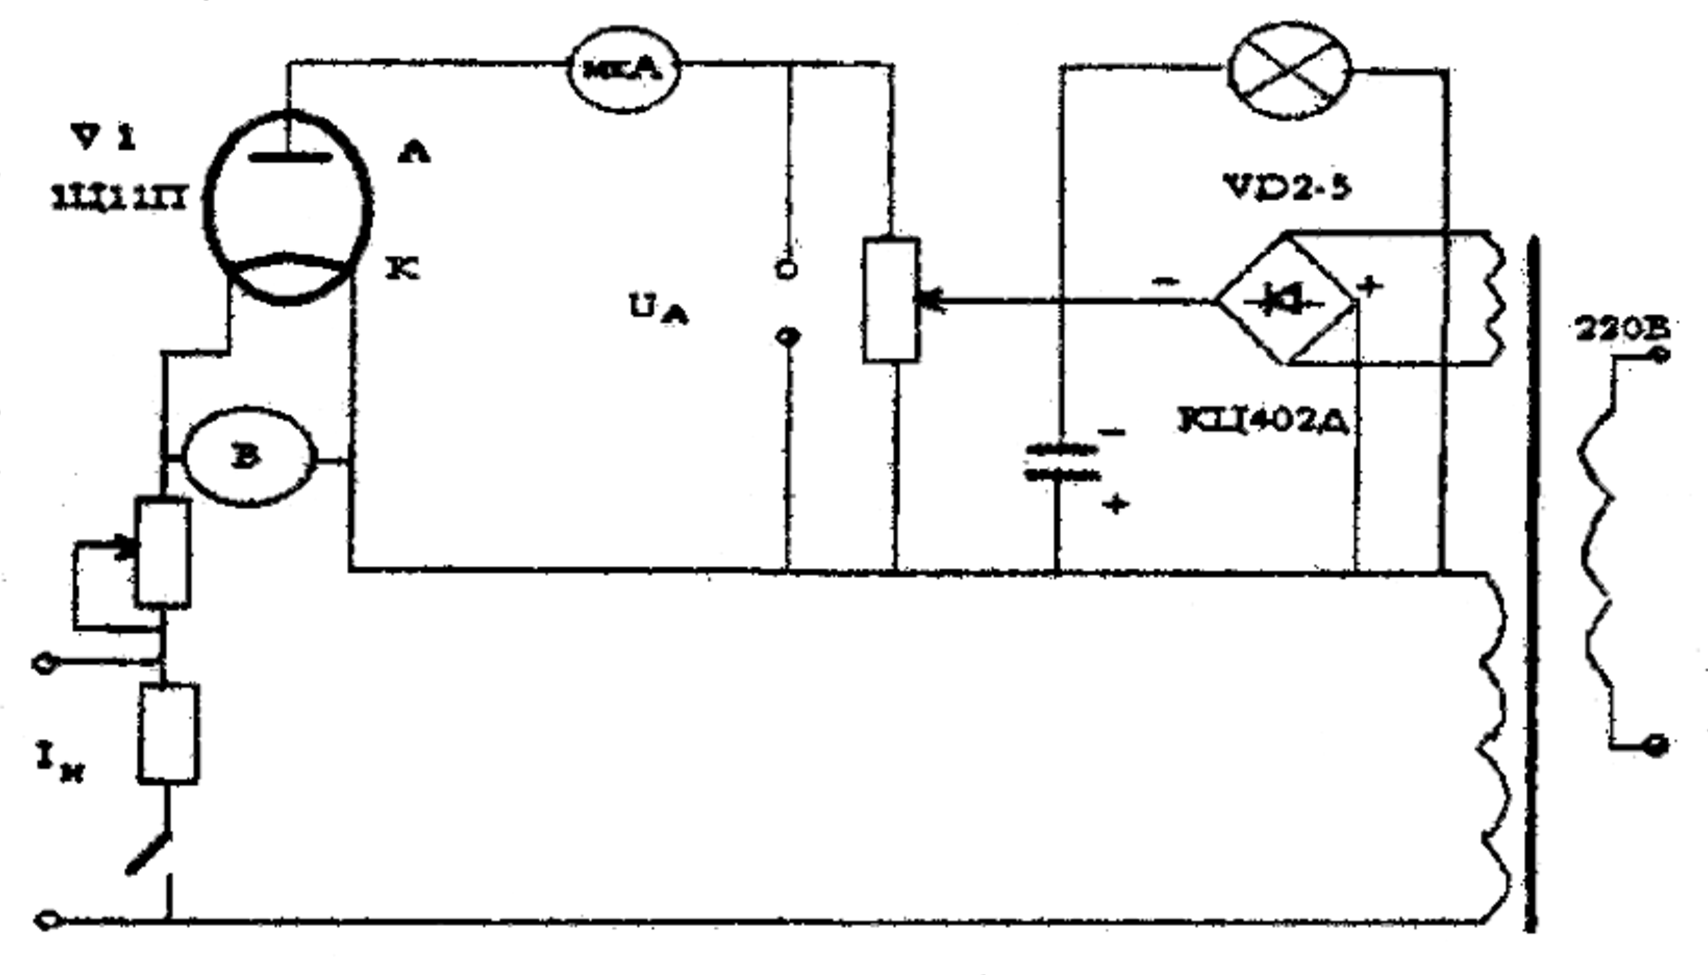
\includegraphics[width=.4\textwidth]{scheme} \hspace*{2em}
        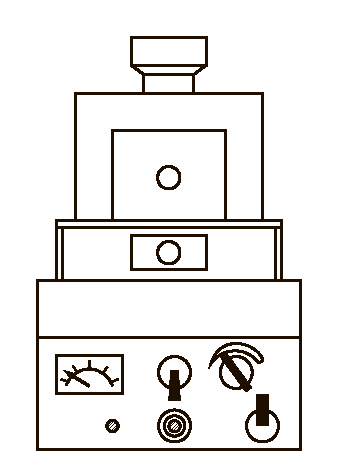
\includegraphics[width=.4\textwidth]{appearance}
    \end{figure} 
    \begin{table}[ht]
        \center
        \caption{Определение температуры катода}
        \begin{tabular}{|C{0.1}|C{0.06}|*{12}{C{.04}|}} \hline
            \multirow{2}{*}{\( U_\textit{н} = 14,\!4 \)~В} &
            \( I_\textit{А} \),~мкА & 0 & 2 & 6 & 8 & 10 & 12 & 14 & 16 & 18 &
            20 & 22 & 24 \\ \cline{2-14}
            & \( U_\textit{А} \),~В & 2,781 & 2,000 & 1,305 & 1,075 & 0,868 &
            0,720 & 0,575 & 0,443 & 0,321 & 0,220 & 0,116 & 0,042 \\ \hline
            \multirow{2}{*}{\( U_\textit{н} = 14,\!8 \)~В} &
            \( I_\textit{А} \),~мкА & 0 & 2 & 8 & 10 & 12 & 14 & 16 & 18 & 20 &
            22 & 24 & 25 \\ \cline{2-14}
            & \( U_\textit{А} \),~В & 2,823 & 2,070 & 1,145 & 0,964 & 0,797 &
            0,654 & 0,512 & 0,394 & 0,291 & 0,188 & 0,100 & 0,045 \\ \hline
            \multirow{2}{*}{\( U_\textit{н} = 15,\!2 \)~В} &
            \( I_\textit{А} \),~мкА & 0 & 2 & 8 & 10 & 12 & 14 & 16 & 18 & 20 &
            22 & 24 & 26 \\ \cline{2-14}
            & \( U_\textit{А} \),~В & 3,000 & 2,160 & 1,219 & 1,016 & 0,857 &
            0,704 & 0,572 & 0,456 & 0,337 & 0,243 & 0,147 & 0,047 \\ \hline
            \multirow{2}{*}{\( U_\textit{н} = 15,\!6 \)~В} &
            \( I_\textit{А} \),~мкА & 0 & 2 & 8 & 10 & 12 & 14 & 18 & 20 & 22 &
            24 & 26 & 28 \\ \cline{2-14}
            & \( U_\textit{А} \),~В & 3,110 & 2,230 & 1,290 & 1,088 & 0,918 &
            0,775 & 0,517 & 0,394 & 0,296 & 0,197 & 0,113 & 0,049 \\ \hline
            \multirow{2}{*}{\( U_\textit{н} = 16,\!0 \)~В} &
            \( I_\textit{А} \),~мкА & 0 & 2 & 8 & 10 & 12 & 14 & 18 & 20 & 22 &
            24 & 26 & 28 \\ \cline{2-14}
            & \( U_\textit{А} \),~В & 3,154 & 2,285 & 1,358 & 1,159 & 0,995 &
            0,837 & 0,570 & 0,452 & 0,355 & 0,253 & 0,158 & 0,051 \\ \hline
            \multirow{2}{*}{\( U_\textit{н} = 16,\!4 \)~В} &
            \( I_\textit{А} \),~мкА & 0 & 2 & 8 & 10 & 12 & 14 & 18 & 20 & 22 &
            24 & 28 & 30 \\ \cline{2-14}
            & \( U_\textit{А} \),~В & 3,240 & 2,400 & 1,430 & 1,230 & 1,045 &
            0,903 & 0,632 & 0,508 & 0,413 & 0,314 & 0,134 & 0,057 \\ \hline
        \end{tabular}
    \end{table}
    
    \begin{table}[h!]
        \center
        \caption{Определение работы выхода}
        \begin{tabular}{|*{7}{C{0.1}|}}\hline
            \(T,\ K\)&&&&&&\\ \hline
            \(I_\textit{А},\ \text{мкА}\)&&&&&&\\ \hline
            \(\ln(I_\textit{А})\)&&&&&&\\ \hline
            
        \end{tabular}
    \end{table}

    \emph{Вывод:}
\end{document}
